\section{Einleitung und Versuchsziel}
\label{sec:aufgabenstellung}
%In der Aufgabenstellung wird (in eigenen Worten und ganzen Sätzen) formuliert, was das Ziel des 
%Versuches ist.  
%[Beachten Sie die eigentliche Aufgabenstellung in den Versuchsanleitungen sowie die Hinweise zur Auswertung!] 

Im folgenden Versuch wird der Azofarbstoff Orange II hergestellt, gereinigt und charakterisiert. Wesentliche Arbeitsmethoden sind bei diesem Versuch das Rühren mittels Magnetrührwerk, das Filtrieren, sowie das Kühlen im Eisbad. Der hergestellte Farbstoff wird mittels Schmelzpunkt und $R_f$-Wert auf seine Reinheit geprüft.\\
Die Reaktionen auf denen die Synthese von Orange II grundsätzlich basiert, sind in Abbildung \ref{fig:reaktion} dargestellt.

\begin{figure}[h!]
	\centering
	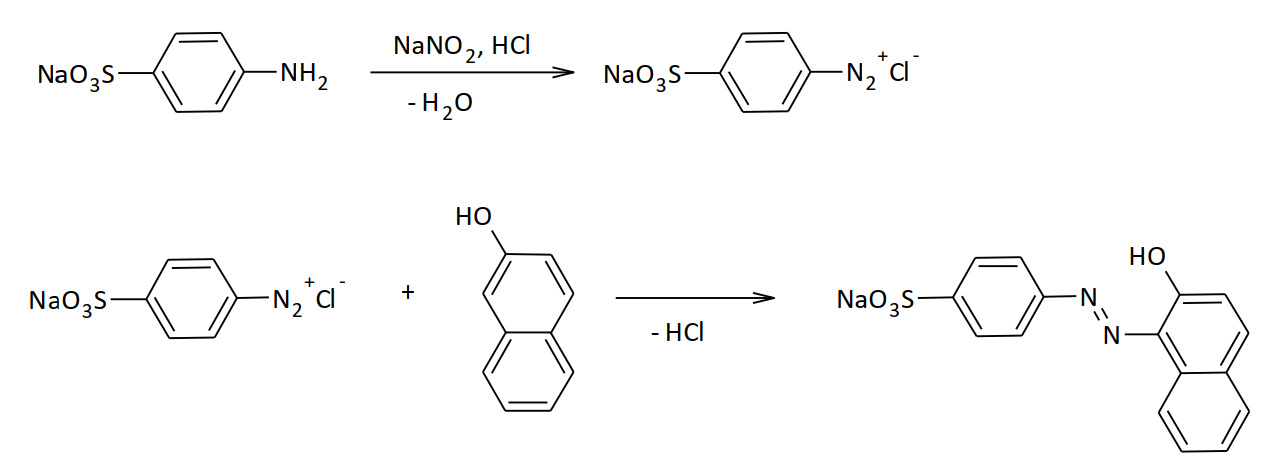
\includegraphics[width=0.9\textwidth]{img/reaktion}
	\caption{Reaktionen zur Synthese von Orange II aus Sulfanilsäure}
	\label{fig:reaktion}
\end{figure}
\FloatBarrier
%Ende